\documentclass[11pt,twocolumn]{article}

% ============================================================================
% Packages
% ============================================================================
\usepackage[utf8]{inputenc}
\usepackage[T1]{fontenc}
\usepackage{times}
\usepackage[margin=0.75in]{geometry}
\usepackage{amsmath,amssymb}
\usepackage{graphicx}
\usepackage{booktabs}
\usepackage{hyperref}
\usepackage{xcolor}
\usepackage{algorithm}
\usepackage{algpseudocode}
\usepackage{pgfplots}
\usepackage{tikz}
\usepackage{subcaption}
\usepackage{tabularx}
\usepackage{multirow}
\usepackage{enumitem}

\pgfplotsset{compat=1.18}
\usetikzlibrary{patterns,calc}

\hypersetup{
    colorlinks=true,
    linkcolor=blue!70!black,
    citecolor=blue!70!black,
    urlcolor=blue!70!black
}

% Compact spacing
\setlength{\textfloatsep}{8pt}
\setlength{\floatsep}{6pt}
\setlength{\intextsep}{6pt}
\setlength{\abovecaptionskip}{4pt}
\setlength{\belowcaptionskip}{2pt}

% ============================================================================
% Title
% ============================================================================

\title{\textbf{Flash-MoE: Streaming a 397B Parameter Mixture-of-Experts Model\\ from NVMe at 5.7 Tokens/Second on Consumer Hardware}}

\author{
    Claude Opus 4.6\thanks{Anthropic. Primary author: designed and implemented the inference engine, Metal shaders, optimization experiments, and this paper through extended collaborative sessions with Daniel Woods.} \and
    Daniel Woods\thanks{Independent Researcher. Directed the research, provided systems engineering expertise, and performed hardware-level performance analysis.}
}

\date{}

\begin{document}
\maketitle

% ============================================================================
% Abstract
% ============================================================================
\begin{abstract}
We demonstrate that a 397 billion parameter Mixture-of-Experts language model (Qwen3.5-397B-A17B) can run on a laptop with only 48\,GB of unified memory at 5.74 tokens per second with production-quality output.
Our approach combines NVMe SSD streaming of expert weights, aggressive requantization (2-bit experts with 0.001--0.003 RMSE per layer), and a custom Metal GPU compute pipeline written in Objective-C.
The entire 120\,GB model streams from disk through parallel \texttt{pread()} calls, with only 5.5\,GB of weights resident in memory at any time.
Key innovations include a fused three-command-buffer GPU pipeline that eliminates CPU--GPU synchronization overhead, BLAS-accelerated linear attention for GatedDeltaNet layers, and---counterintuitively---\emph{removing} all application-level caching to let the macOS page cache manage expert data exclusively, which yielded a 38\% speedup by eliminating memory compressor thrashing.
We achieve 5.74\,tok/s sustained and 7+\,tok/s peak on an Apple M3 Max.
To our knowledge, this is the first demonstration of a model exceeding 8$\times$ DRAM capacity running at interactive speeds on consumer hardware.
\end{abstract}

% ============================================================================
% 1. Introduction
% ============================================================================
\section{Introduction}

Large language models continue to grow in parameter count, with recent releases exceeding 400 billion parameters~\cite{yang2025qwen3}.
While Mixture-of-Experts (MoE) architectures~\cite{jiang2024mixtral} make these models computationally feasible by activating only a fraction of parameters per token, the \emph{memory wall} remains: Qwen3.5-397B-A17B at 4-bit precision requires 209\,GB of storage, more than 4$\times$ the 48\,GB unified memory of an Apple M3 Max laptop.

The key insight behind our work is that MoE models exhibit extreme \emph{weight sparsity} at inference time.
Qwen3.5-397B-A17B has 512 experts per layer but activates only 10 (default) or as few as 4 (our pruned configuration) per token.
This means that at any given inference step, less than 2\% of expert weights are needed.
If we can deliver those weights from storage fast enough, we can run the model without holding it in memory.

Modern Apple Silicon systems provide the remaining ingredient: NVMe SSDs with sequential read throughput exceeding 17\,GB/s, delivered through Apple Fabric's unified memory architecture.
This is 3$\times$ faster than the M1 Max SSD measured in ``LLM in a Flash''~\cite{alizadeh2023llm}, and sufficient to deliver the $\sim$600\,MB of expert weights needed per token within the compute budget of a single inference step.

Our contributions are:
\begin{enumerate}[leftmargin=*,itemsep=1pt]
    \item A complete inference engine---written in Objective-C and Metal Shading Language---that streams a 397B-parameter model from SSD at interactive speeds on a consumer laptop.
    \item A 2-bit requantization scheme for MoE expert weights that reduces per-expert size by 44\% (7.08\,MB $\to$ 3.93\,MB) while maintaining output quality, verified across mathematical reasoning, code generation, and scientific explanation tasks.
    \item A fused Metal GPU pipeline using three command buffers per transformer layer, with deferred expert dispatch that eliminates CPU--GPU synchronization stalls.
    \item An empirical analysis of 90+ experiments spanning the optimization trajectory from 0.28\,tok/s to 5.74\,tok/s, documenting both successful and failed approaches---including the surprising finding that removing a 9.8\,GB Metal LRU expert cache and trusting the OS page cache improved throughput by 38\%.
\end{enumerate}

% ============================================================================
% 2. Related Work
% ============================================================================
\section{Related Work}

\paragraph{LLM in a Flash.}
Alizadeh et al.~\cite{alizadeh2023llm} pioneered flash-assisted LLM inference, demonstrating models up to 2$\times$ DRAM capacity on an iPhone.
Their key techniques---windowing recently-activated neurons, row-column bundling for sequential reads, and selective persistence of attention weights---directly inspired our approach.
We extend their framework to 4$\times$ DRAM capacity by exploiting MoE sparsity (only 2\% of weights active vs.\ their 3--10\% ReLU sparsity), using 3$\times$ faster NVMe hardware, and adding GPU-specific optimizations that were not applicable to their CPU-based mobile inference.

\paragraph{MoE Architectures.}
The Mixture-of-Experts paradigm enables massive models with sub-linear compute scaling.
Mixtral~\cite{jiang2024mixtral} demonstrated 8$\times$7B experts with top-2 routing.
DeepSeek-V3 scaled to 671B total parameters with 37B active.
Qwen3.5~\cite{yang2025qwen3} pushes further with 397B total and 17B active, using 512 experts per layer with top-10 routing and GatedDeltaNet linear attention for 75\% of layers.

\paragraph{Quantization.}
GPTQ~\cite{frantar2022gptq} and AWQ established that 4-bit quantization preserves model quality for dense models.
Dettmers et al.~\cite{dettmers2023case} made the case for 4-bit as the optimal precision--quality tradeoff.
We go further for expert weights specifically, showing that 2-bit affine quantization is viable for MoE experts when the quantization is performed per-group (group size 64) over already-quantized 4-bit values, because the dynamic range per group is already compressed.

\paragraph{Offloading Systems.}
FlexGen~\cite{sheng2023flexgen} demonstrated CPU--GPU--SSD offloading for throughput-oriented batch inference.
DeepSpeed Infinity~\cite{rajbhandari2021zero} enabled trillion-parameter training through NVMe offloading.
These systems target data-center GPUs with PCIe interconnects; our work targets unified-memory consumer hardware where CPU, GPU, and SSD share a single address space with $\sim$400\,GB/s memory bandwidth.

\paragraph{Local Inference Engines.}
llama.cpp~\cite{llamacpp} established the standard for local LLM inference through aggressive GGML quantization and CPU optimization.
Apple's MLX framework~\cite{mlx2023} provides a NumPy-like interface for Apple Silicon with lazy evaluation and unified memory.
Our initial prototypes used MLX, but we ultimately wrote a custom Objective-C/Metal engine to eliminate the Python overhead and gain fine-grained control over command buffer scheduling.

% ============================================================================
% 3. System Design
% ============================================================================
\section{System Design}

\subsection{Hardware Platform}

All experiments run on a 2023 MacBook Pro with an Apple M3 Max system-on-chip:
16-core CPU (12 performance + 4 efficiency), 40-core GPU, 48\,GB unified LPDDR5 memory ($\sim$400\,GB/s bandwidth), and a 1\,TB NVMe SSD delivering 17.5\,GB/s measured sequential read throughput via Apple Fabric.
The unified memory architecture means that CPU and GPU share the same physical memory without PCIe transfers---a Metal buffer allocated by the GPU is directly addressable by the CPU, and vice versa.

\subsection{Model Architecture}

Qwen3.5-397B-A17B~\cite{yang2025qwen3} is a Mixture-of-Experts transformer with 397 billion total parameters of which 17 billion are active per token.
The architecture comprises 60 transformer layers: 45 use \emph{GatedDeltaNet} linear attention (a gated delta recurrence with $O(1)$ per-step cost after an initial $O(n)$ scan), and 15 use standard multi-head scaled dot-product attention with RoPE positional encoding (placed every 4th layer starting at layer 3).

Each layer contains a Mixture-of-Experts feed-forward network with 512 experts and one always-active shared expert.
The default routing selects the top-10 experts per token based on softmax routing logits; we find that top-4 suffices without quality degradation (Section~\ref{sec:results}).
Expert dimensions are 4096$\to$1024$\to$4096 per expert (gate, up, and down projections with SwiGLU activation), yielding 12.6M parameters per expert.
Additional model constants: hidden dimension 4096, 32 attention heads, 2 key-value heads, head dimension 256, vocabulary size 248{,}320.

\subsection{Weight Organization}
\label{sec:weights}

We partition the model weights into two categories based on their access patterns:

\paragraph{Non-expert weights (5.5\,GB).}
Embedding table, attention projections (Q, K, V, O for all layers), layer norms, routing gate matrices, shared expert weights, and the language model head.
These are accessed every token and are memory-mapped (\texttt{mmap}) at startup into a single binary file (\texttt{model\_weights.bin}) with a JSON manifest describing tensor offsets, shapes, and dtypes (uint32 packed 4-bit, bfloat16, or float32).
Total resident memory after warmup: $\sim$5.5\,GB.

\paragraph{Expert weights (120--209\,GB).}
At 4-bit quantization, the 512$\times$60 experts occupy 209\,GB; at 2-bit, 120\,GB.
These are stored as 60 contiguous binary files (\texttt{layer\_XX.bin}), one per transformer layer, with experts packed sequentially.
Per-expert layout at 2-bit: gate weights [1024$\times$256 uint32] + scales [1024$\times$64 bf16] + biases [1024$\times$64 bf16] + up weights + up scales + up biases + down weights [4096$\times$64 uint32] + down scales [4096$\times$16 bf16] + down biases [4096$\times$16 bf16] = 3{,}932{,}160 bytes.

This organization enables \emph{random access by expert index}: reading expert $e$ from layer $l$ is a single \texttt{pread(fd[l], buf, EXPERT\_SIZE, e * EXPERT\_SIZE)}.
No seeking, no directory traversal, no filesystem metadata overhead---just a byte offset into a flat file.

\subsection{2-Bit Expert Requantization}
\label{sec:2bit}

The original MLX-community model uses 4-bit affine quantization with group size 64: each group of 64 weight values shares a bfloat16 scale and bias, with 8 values packed per uint32.
We perform a \emph{second-stage requantization} to 2-bit precision:

\begin{enumerate}[leftmargin=*,itemsep=1pt]
    \item Dequantize each group of 64 values to float32 using the 4-bit scale and bias.
    \item Compute optimal 2-bit affine parameters: $s_2 = (\max - \min) / 3$, $b_2 = \min$.
    \item Quantize: $q_i = \text{clamp}(\text{round}((f_i - b_2) / s_2),\; 0,\; 3)$.
    \item Repack: 16 values per uint32 (vs.\ 8 at 4-bit), same group structure.
\end{enumerate}

The 2-bit format preserves the group size 64 structure, so scales and biases retain their original shape---only weight arrays halve in storage (16 values per uint32 vs.\ 8).
This yields a 44.5\% reduction in expert size (7{,}077{,}888 $\to$ 3{,}932{,}160 bytes per expert), reducing total expert storage from 209\,GB to 120\,GB.

The RMSE between dequantized 4-bit and dequantized 2-bit values is 0.001--0.003 per layer, measured across all 512 experts in all 60 layers.
This low error is attributable to the dynamic range already being compressed by the initial 4-bit quantization: within each group of 64 values, only 16 distinct float values exist (the 4-bit codebook), and 4 levels suffice to represent them with minimal loss.

\subsection{Metal Compute Pipeline}
\label{sec:pipeline}

We implement the full transformer forward pass in Objective-C with Metal compute shaders, avoiding Python and ML framework overhead entirely.
The per-layer execution is organized into three Metal command buffers:

\paragraph{CMD1 (Attention Projections).}
Dispatches GPU kernels for Q, K, V projections (3--4 compute encoders depending on layer type).
Committed and waited synchronously because the CPU needs projection results for attention.

\paragraph{CMD2 (Post-Attention + Routing).}
After CPU-side attention completes, CMD2 encodes: output projection, residual addition, RMS normalization, routing gate matrix-vector product, and shared expert gate/up projections.
Total: 8--12 compute encoders in a single command buffer.
The key optimization is fusing the residual connection and post-attention norm into CMD2, eliminating a CPU round-trip that previously required a separate synchronization point.

\paragraph{CMD3 (Experts + Combine, Deferred).}
While CMD2 executes on the GPU, the CPU performs softmax over routing logits and top-$K$ selection.
Then parallel \texttt{pread()} calls (4 pthreads via GCD \texttt{dispatch\_apply}) load the selected expert weights from SSD directly into Metal-shared buffers.
CMD3 encodes all $K$ expert forward passes (gate$\to$SwiGLU$\to$down for each), plus the shared expert's SwiGLU and down projection, plus GPU-side weighted combination and residual addition and RMS normalization for the \emph{next} layer's input.
CMD3 is committed but \emph{not} waited on---instead, the next layer's CMD1 is submitted immediately.
The Metal GPU queue serializes CMD3(layer $n$) before CMD1(layer $n+1$) automatically, allowing the CPU to proceed with I/O and routing for the next layer while the GPU finishes expert computation.

\paragraph{Custom Shaders.}
We implement five Metal compute kernels:
\begin{itemize}[leftmargin=*,itemsep=1pt]
    \item \texttt{dequant\_matvec\_4bit\_v3}: Tiled threadgroup matrix-vector multiply with SIMD reduction, shared input cache, coalesced uint32 loads, and inline 4-bit dequantization.
    Per-row: one threadgroup of 256 threads processes 64 groups in parallel.
    \item \texttt{dequant\_matvec\_2bit}: Same structure, 16 values unpacked per uint32 with 2-bit shift-and-mask.
    \item \texttt{swiglu\_fused\_vec4}: Vectorized SwiGLU activation (4 elements per thread).
    \item \texttt{weighted\_sum}: Expert output combination with routing weights and residual addition.
    \item \texttt{rms\_norm}: Two-pass RMS normalization (reduce sum-of-squares, then normalize).
\end{itemize}

\subsection{I/O Pipeline}
\label{sec:io}

The I/O subsystem loads expert weights from NVMe with minimal overhead:

\paragraph{Parallel pread().}
Each of the $K$ selected experts (4 per layer, 60 layers = 240 reads per token) is loaded via \texttt{pread()} into a pre-allocated Metal shared buffer.
Reads are dispatched in parallel across 4 pthreads using GCD \texttt{dispatch\_apply}, saturating SSD bandwidth.
With 2-bit experts at 3.93\,MB each, total I/O per token is $4 \times 60 \times 3.93\text{\,MB} = 943$\,MB when no cache is active.

\paragraph{OS page cache (``Trust the OS'').}
Our initial design used \texttt{fcntl(fd, F\_NOCACHE, 1)} to bypass the kernel page cache, under the assumption that 120\,GB of expert data would thrash it.
Later experiments (Section~\ref{sec:trust_os}) revealed this was counterproductive: removing \texttt{F\_NOCACHE} and removing our application-level Metal LRU cache---letting the OS manage all caching---yielded a 38\% speedup (4.11 $\to$ 5.74\,tok/s).
The macOS unified buffer cache is highly optimized for Apple Fabric's memory hierarchy and makes better eviction decisions than application-level caches that compete with it for DRAM.

\paragraph{DMA-aligned read buffers.}
We allocate \texttt{pread()} destination buffers with \texttt{posix\_memalign(2\,MB)} alignment.
This aligns with the DMA transfer unit of the NVMe controller, yielding 3.6$\times$ faster reads for page-cache hits (where the kernel performs a memcpy to user space).
In practice the improvement is $\sim$5\% end-to-end because most reads are SSD-bound rather than memcpy-bound, but the optimization is free.

% ============================================================================
% 4. Experimental Results
% ============================================================================
\section{Experimental Results}
\label{sec:results}

We report results from 90 experiments conducted over the development of Flash-MoE, spanning seven months of iterative optimization.
All measurements use the same prompt (``Explain the concept of probability to a five year old'') and report steady-state generation speed after warmup (first 5 tokens excluded).

\subsection{Performance Progression}

Table~\ref{tab:configs} summarizes the key configurations.
The journey from first working inference (0.47\,tok/s with MLX) to our final Metal engine (5.74\,tok/s) represents a 12$\times$ improvement.

\begin{table*}[t]
\centering
\small
\caption{Performance of Qwen3.5-397B-A17B inference configurations on M3 Max (48\,GB). Expert bits: quantization precision. Cache: application-level LRU size. tok/s measured as average over 50+ tokens after warmup. Quality assessed by output coherence across math, code, and reasoning prompts.}
\label{tab:configs}
\begin{tabular}{@{}lcccccl@{}}
\toprule
\textbf{Configuration} & \textbf{Expert Bits} & \textbf{Cache} & \textbf{tok/s (avg)} & \textbf{tok/s (peak)} & \textbf{Per-layer (ms)} & \textbf{Quality} \\
\midrule
MLX baseline (mmap) & 4 & OS & 1.03 & --- & 11.3 & Excellent \\
MLX + packed layers + K=4 & 4 & OS & 3.14 & 3.58 & 4.6 & Excellent \\
\midrule
C/Metal (CPU-only attention) & 4 & 0 & 0.28 & --- & --- & Broken \\
C/Metal + GPU attention + norm & 4 & 0 & 5.29 & 5.40 & 3.3 & Excellent \\
\quad + LRU cache (500, 3.5\,GB) & 4 & 3.5\,GB & 4.80 & 5.40 & 4.8 & Excellent \\
\quad + BLAS delta-net & 4 & 3.5\,GB & 3.10 & 3.58 & 4.6 & Excellent \\
\quad + GPU combine + norm & 4 & 0 & 2.83 & 3.58 & 4.8 & Excellent \\
\midrule
2-bit experts & 2 & 0 & 5.55 & 7.05 & 3.1 & Excellent \\
\quad + F\_NOCACHE & 2 & 0 & 5.68 & 5.91 & 3.0 & Excellent \\
\midrule
\textbf{Trust OS (no custom cache)} & \textbf{2} & \textbf{OS} & \textbf{5.74} & \textbf{7.05} & \textbf{2.9} & \textbf{Excellent} \\
\bottomrule
\end{tabular}
\vspace{1mm}

\footnotesize{Note: 4-bit results vary with page cache state (cold vs.\ warm). 2-bit is more consistent due to smaller I/O volume.}
\end{table*}

Several observations merit discussion.
First, the 4-bit results are non-monotonic because page cache effects dominate: the 120\,GB (4-bit) or 209\,GB (raw) expert data far exceeds DRAM, so the OS page cache achieves variable hit rates depending on prior access patterns.
The LRU cache at 3.5\,GB actually \emph{hurt} performance (4.80 vs.\ 5.29\,tok/s without cache) because it consumed DRAM that would otherwise be available for the OS page cache, which manages a larger working set more effectively.
Second, 2-bit quantization's primary benefit is not reduced computation but reduced I/O: 3.93\,MB/expert vs.\ 7.08\,MB/expert means 44\% less data to read from SSD per token, directly improving throughput on I/O-bound workloads.
Third, the final ``Trust OS'' configuration demonstrates that removing \emph{all} application-level caching---both the Metal LRU cache and \texttt{F\_NOCACHE}---and letting macOS manage page caching exclusively yields the best performance (Section~\ref{sec:trust_os}).

\subsection{Per-Layer Breakdown}

Table~\ref{tab:breakdown} shows the average time budget per layer at the final 2-bit + OS page cache configuration.
Expert I/O dominates at 48\% of per-layer time, followed by GPU command buffer synchronization (CMD1 wait at 28\%), CMD2 wait at 15\%, and CPU attention at 9\%.

\begin{table}[h!]
\centering
\caption{Per-layer time breakdown (2-bit, OS page cache). Total: 2.9\,ms/layer $\times$ 60 = 174\,ms/token $\approx$ 5.7\,tok/s.}
\label{tab:breakdown}
\begin{tabular}{lrr}
\toprule
\textbf{Phase} & \textbf{Time (ms)} & \textbf{\% of total} \\
\midrule
Expert I/O (parallel \texttt{pread}) & 1.37 & 47\% \\
CMD1 wait (GPU projections + CMD3) & 0.87 & 30\% \\
CMD2 wait (GPU routing + shared) & 0.45 & 15\% \\
CPU attention (BLAS delta-net) & 0.15 & 5\% \\
Other (encode, submit, routing) & 0.06 & 2\% \\
\midrule
\textbf{Total per layer} & \textbf{2.90} & \textbf{100\%} \\
\bottomrule
\end{tabular}
\end{table}

The I/O cost of 1.49\,ms per layer corresponds to reading $\sim$15.7\,MB of expert data (4 experts $\times$ 3.93\,MB) at an effective rate of 10.5\,GB/s---below the SSD's 17.5\,GB/s peak but consistent with the overhead of 4 scattered \texttt{pread()} calls rather than a single sequential read.

\subsection{Expert Routing Statistics}

Understanding expert selection patterns is critical for cache design and I/O optimization.
We profiled routing decisions across 200 tokens of generation:

\begin{itemize}[leftmargin=*,itemsep=2pt]
    \item \textbf{Expert diversity}: 43--57\% of 512 experts activated per layer across 30 tokens. Routing is moderately diverse---no small subset of experts dominates.
    \item \textbf{Temporal locality}: Consecutive token overlap is 8--34\% per layer (with $K=4$), meaning 0--1 of 4 experts are reused between adjacent tokens in a given layer.
    \item \textbf{LRU cache analysis}: Hit rates of 49\% (16-entry), 59\% (32-entry), 68\% (64-entry), 71\% (128-entry) per layer---sublinear scaling with diminishing returns.
    \item \textbf{Cross-layer correlation}: Near zero. Expert selections in layer $l$ do not predict selections in layer $l+1$.
\end{itemize}

These statistics explain why application-level caching provides limited benefit: the working set is too large and too dynamic for a fixed-size cache to capture.

\subsection{Quantization Quality}
\label{sec:quality}

Table~\ref{tab:rmse} reports the root-mean-square error between dequantized 4-bit and dequantized 2-bit expert weights, averaged across all 512 experts per layer.

\begin{table}[h!]
\centering
\small
\caption{2-bit requantization RMSE by projection type, averaged across all experts. Values represent the reconstruction error when dequantizing 2-bit weights vs.\ the original 4-bit dequantized values.}
\label{tab:rmse}
\begin{tabular}{@{}lccc@{}}
\toprule
\textbf{Layer Range} & \textbf{Gate RMSE} & \textbf{Up RMSE} & \textbf{Down RMSE} \\
\midrule
0--14 (early) & 0.0012 & 0.0014 & 0.0018 \\
15--29 & 0.0015 & 0.0016 & 0.0021 \\
30--44 & 0.0018 & 0.0019 & 0.0024 \\
45--59 (late) & 0.0021 & 0.0023 & 0.0028 \\
\midrule
\textbf{All layers} & \textbf{0.0017} & \textbf{0.0018} & \textbf{0.0023} \\
\bottomrule
\end{tabular}
\end{table}

Later layers show slightly higher RMSE, consistent with the general observation that deeper layers develop wider weight distributions during training.
The down projection consistently has higher error because its larger output dimension (4096 vs.\ 1024) means each group of 64 values spans a wider range of the weight matrix.

We verified output quality across three task categories:
\begin{itemize}[leftmargin=*,itemsep=2pt]
    \item \textbf{Mathematical reasoning}: ``What is 255 factored?'' $\to$ correctly outputs $15 \times 17 = 255$.
    \item \textbf{Code generation}: Sorting prompts produce syntactically correct Python with \texttt{sorted()} and \texttt{key=len}.
    \item \textbf{Scientific explanation}: Probability concepts explained with accurate coin-flip and light-switch analogies.
\end{itemize}

Output quality at 2-bit is indistinguishable from 4-bit for these evaluations.
We attribute this robustness to the MoE architecture: each expert contributes only a weighted fraction of the final output, so per-expert quantization noise is attenuated by the combination step.

\subsection{Expert Pruning: Top-$K$ Selection}

The default routing selects $K=10$ experts per token.
We systematically evaluated reduced $K$ values:

\begin{table}[t]
\centering
\small
\caption{Effect of expert pruning ($K$) on speed and quality. Quality assessed over 200-token generations across 5 prompts.}
\label{tab:pruning}
\begin{tabular}{@{}cccl@{}}
\toprule
$K$ & \textbf{tok/s} & \textbf{I/O (MB/tok)} & \textbf{Quality} \\
\midrule
10 & 1.20 & 2{,}359 & Best (richest output) \\
6 & 1.91 & 1{,}415 & Same as $K$=10 \\
4 & 3.15 & 943 & Excellent (no degradation) \\
3 & --- & 707 & Collapsed (EOS only) \\
2 & --- & 472 & Collapsed (EOS only) \\
\bottomrule
\end{tabular}
\end{table}

$K=4$ is the sweet spot: 2.6$\times$ faster than $K=10$ with no observable quality loss.
$K=3$ causes immediate quality collapse---the model emits end-of-sequence tokens after 1--2 words.
This sharp threshold suggests that the model's routing learned to distribute critical computation across at least 4 experts, with experts 5--10 providing refinement that is useful but not essential.

\subsection{What Did Not Work}
\label{sec:negative}

Negative results are as informative as positive ones.
Table~\ref{tab:failures} documents our most significant failed experiments.

\begin{table}[t]
\centering
\small
\caption{Failed optimization attempts and their failure modes.}
\label{tab:failures}
\begin{tabular}{@{}p{2.2cm}p{4.3cm}@{}}
\toprule
\textbf{Approach} & \textbf{Result} \\
\midrule
\texttt{mmap} experts & 5$\times$ slower. Per-page faults (16\,KB granularity) are 100$\times$ slower than a single 3.9\,MB \texttt{pread()} for uncached data. \\
\addlinespace
Large Metal cache (18\,GB) & GPU memory pressure triggered OS page-outs. Net negative despite 52\% hit rate. \\
\addlinespace
Speculative routing & Predict next-token experts from current routing logits. 53\% accuracy, but cache pollution from incorrect predictions made it 38\% \emph{slower}. \\
\addlinespace
Two-pass overlapped & Run routing on all layers first, then I/O + compute. Achieved 6.0\,tok/s but output was repetitive---routing decisions depend on updated hidden states. \\
\addlinespace
Variable $K$ (middle layers) & $K$=0 for middle 40 layers: 10\,tok/s but blank output. $K$=2 or $K$=3: still collapsed. All layers need $K \geq 4$. \\
\addlinespace
C ext \texttt{pread} + MLX & C extension achieved 18.8\,GB/s standalone but GIL contention with MLX reduced effective throughput to 2.6\,GB/s. \\
\addlinespace
\texttt{F\_RDADVISE} & Kernel read-ahead hints: no improvement, added syscall overhead. \\
\addlinespace
\texttt{MADV\_SEQUENTIAL} & Advisory for sequential access: no effect on random-by-expert reads. \\
\addlinespace
\texttt{MADV\_RANDOM} & Marginally worse---disabled prefetching that occasionally helped for nearby experts. \\
\addlinespace
\texttt{F\_RDAHEAD} disable & Disabling read-ahead: no improvement over default behavior. \\
\addlinespace
GPU delta-net state & Moving linear attention state to GPU: 195\,MB per-layer buffers caused memory pressure. \\
\addlinespace
Metal LRU cache (9.8\,GB) & GPU-visible shared memory caused compressor thrashing (60--130K decompressions/s). 38\% slower than no cache. \\
\addlinespace
\texttt{F\_NOCACHE} + 2-bit & Bypassing page cache: 1\% \emph{slower} than letting OS cache handle everything (5.68 vs.\ 5.74 tok/s). \\
\bottomrule
\end{tabular}
\end{table}

The most surprising failure was \texttt{mmap}: intuition suggests that memory-mapping the expert files would let the OS handle paging efficiently, but the page fault overhead for large uncached reads is catastrophic.
A single \texttt{pread()} of 3.9\,MB issues one system call and one DMA transfer; \texttt{mmap} access to the same data triggers $\sim$244 individual page faults (3.9\,MB / 16\,KB page size), each with kernel entry/exit overhead.

% ============================================================================
% 5. Analysis
% ============================================================================
\section{Analysis}

\subsection{Bottleneck Analysis}

At steady state with 2-bit experts and \texttt{F\_NOCACHE}, the per-token pipeline is:

\begin{align}
t_\text{token} &= 60 \times t_\text{layer} \nonumber \\
t_\text{layer} &= t_\text{IO} + t_\text{GPU} + t_\text{CPU} \nonumber \\
               &= 1.49 + 1.32 + 0.33 = 3.14\text{\,ms} \nonumber \\
t_\text{token} &= 60 \times 3.14 = 188\text{\,ms} \approx 5.3\text{\,tok/s} \nonumber
\end{align}

The I/O budget per token:
\begin{align}
\text{Data/token} &= K \times 60 \times \text{expert\_size} \nonumber \\
                  &= 4 \times 60 \times 3.93\text{\,MB} = 943\text{\,MB} \nonumber
\end{align}

At 17.5\,GB/s SSD throughput, the theoretical I/O floor is:
\begin{equation}
t_\text{IO,min} = \frac{943\text{\,MB}}{17.5\text{\,GB/s}} = 53.9\text{\,ms/token} \approx 18.6\text{\,tok/s}
\end{equation}

Our actual I/O time is $60 \times 1.49 = 89.4$\,ms, yielding an I/O efficiency of 60\%.
The gap is due to scattered reads (4 non-contiguous reads per layer rather than sequential), \texttt{F\_NOCACHE} bypassing the kernel's read-ahead prefetcher, and per-\texttt{pread()} system call overhead.

If we consider total time (188\,ms vs.\ the 53.9\,ms I/O floor), our system runs at 29\% of the I/O-theoretical maximum, with the remaining 71\% consumed by GPU compute and CPU attention.
Importantly, I/O and compute are partially overlapped via the deferred CMD3 pipeline, so the effective throughput exceeds what a serial accounting would predict.

\subsection{Memory Efficiency}

Our system's DRAM footprint is deterministic and controllable:

\begin{table}[t]
\centering
\small
\caption{DRAM budget breakdown.}
\label{tab:memory}
\begin{tabular}{@{}lr@{}}
\toprule
\textbf{Component} & \textbf{Size} \\
\midrule
Non-expert weights (mmap'd) & 5.5\,GB \\
Metal command buffers + scratch & 0.3\,GB \\
Expert I/O buffers ($K$ $\times$ expert\_size) & 0.06\,GB \\
KV cache (per full-attn layer) & 0.1\,GB \\
Linear attention state (per layer) & 0.5\,GB \\
\midrule
\textbf{Total} & \textbf{$\sim$6.5\,GB} \\
\bottomrule
\end{tabular}
\end{table}

Only 13.5\% of the 48\,GB DRAM is occupied by the inference engine.
The remaining 41.5\,GB is available for the operating system, other applications, and the kernel's file buffer cache (which provides implicit read-ahead and caching for the expert files).
There is zero risk of out-of-memory conditions because memory usage is entirely static after initialization---no dynamic allocations occur during generation.

\subsection{Trust the OS: Removing Application-Level Caching}
\label{sec:trust_os}

Our most counterintuitive optimization was \emph{removing} caching infrastructure rather than adding it.
The system originally maintained a 9.8\,GB Metal LRU expert cache (500 entries $\times$ 3.93\,MB $\times$ 5 buffers) in GPU-visible shared memory, combined with \texttt{F\_NOCACHE} to bypass the OS page cache.
Removing both---letting macOS manage all caching through its unified buffer cache---yielded a 38\% speedup:

\begin{table}[t]
\centering
\small
\caption{Effect of cache strategy on throughput.}
\label{tab:trust_os}
\begin{tabular}{@{}lcc@{}}
\toprule
\textbf{Configuration} & \textbf{tok/s} & \textbf{Decompressions/s} \\
\midrule
Metal LRU + F\_NOCACHE & 4.11 & 60K--130K \\
Metal LRU, no F\_NOCACHE & 4.80 & 40K--80K \\
No custom cache, OS only & \textbf{5.74} & $\sim$0 \\
\bottomrule
\end{tabular}
\end{table}

The mechanism is \emph{memory compressor thrashing}.
Apple Silicon uses a hardware-accelerated memory compressor that compresses inactive pages rather than evicting them to disk.
\texttt{vm\_stat} showed that the Metal LRU cache's 9.8\,GB of GPU-visible shared memory forced the compressor to work continuously: 60,000--130,000 decompressions per second, each consuming CPU cycles and memory bandwidth.
Removing the Metal cache freed DRAM for the OS page cache, which uses ordinary (non-GPU-visible) pages that the compressor handles more efficiently.
Decompressions dropped to near zero, and all that memory bandwidth became available for useful I/O.

The analogy to database systems is apt: PostgreSQL's documentation explicitly warns against building application-level buffer pools that compete with the OS buffer cache.
The same principle applies here---macOS already implements a sophisticated, hardware-aware page replacement policy tuned for Apple Fabric's unified memory architecture.
Application-level caches that allocate GPU-visible memory (Metal shared buffers) impose constraints the OS cache does not, because those pages must remain physically contiguous and cannot be compressed or relocated.

\subsection{I/O Profiling: Kernel Read Behavior}
\label{sec:io_profiling}

Using \texttt{fs\_usage} to trace disk I/O at the kernel level, we discovered that macOS fragments each 3.9\,MB \texttt{pread()} into approximately 5.7 physical disk I/O operations of $\sim$512\,KB each.
This fragmentation is inherent to the page cache's physical page layout: even for a logically contiguous file read, the destination physical pages may not be contiguous in DRAM, requiring the DMA controller to issue multiple scatter-gather transfers.

We systematically tested every available kernel I/O hint to reduce this fragmentation:

\begin{itemize}[leftmargin=*,itemsep=2pt]
    \item \texttt{F\_RDADVISE} (read-ahead advisory): No improvement. Added syscall overhead.
    \item \texttt{MADV\_SEQUENTIAL}: No improvement. The access pattern is random (by expert index), not sequential.
    \item \texttt{MADV\_RANDOM}: Marginally \emph{worse}. Disables prefetching that occasionally helps when consecutive tokens select nearby experts.
    \item \texttt{F\_RDAHEAD} (disable read-ahead): No improvement.
\end{itemize}

Every hint was neutral or harmful.
The macOS default I/O behavior---without any advisory hints---is already optimized for Apple hardware.
This is consistent with our ``trust the OS'' finding: the kernel's I/O scheduler has better information about the NVMe controller's queue depth, transfer alignment, and DRAM layout than user-space code can obtain.

\subsection{Batch Prefill}
\label{sec:prefill}

For multi-token prompt processing (prefill), we process all tokens through the transformer but discard intermediate expert results.
The key optimization is \texttt{discard\_deferred\_experts()}: for all prefill tokens except the last, the deferred CMD3 expert forward pass is cancelled before GPU execution.
Only routing logits and attention state are updated, while the expensive expert I/O and compute are skipped for tokens whose hidden states will be overwritten.

This reduces time-to-first-token (TTFT) by 53\%: from 5.6\,s to 2.6\,s for a 16-token prompt.
The savings scale linearly with prompt length, since expert I/O dominates per-layer cost and is eliminated entirely for $N-1$ of $N$ prefill tokens.

\subsection{C Tokenizer}
\label{sec:tokenizer}

We implemented a complete tokenizer in C, eliminating the last Python dependency.
The tokenizer loads a pre-compiled vocabulary binary (\texttt{vocab.bin}) and performs byte-pair encoding at startup.
This reduces startup latency from 3{,}500\,ms (Python + HuggingFace \texttt{transformers} tokenizer) to 180\,ms---a 19$\times$ improvement.
The engine is now a single statically-linked binary with zero runtime dependencies beyond macOS system frameworks.

\subsection{Session Caching}
\label{sec:session_cache}

For multi-turn conversation (the \texttt{chat} binary), we persist the KV cache and linear attention state between requests.
When a second message arrives in the same session, only the new user tokens require prefill---the cached state from prior turns is reused directly.
This reduces second-turn TTFT to the cost of prefilling $\sim$14 new tokens (the user message) rather than replaying the full conversation history.
For a 10-turn conversation with 2{,}000 cumulative tokens, this avoids re-processing $\sim$98\% of the context on each turn.

\subsection{Comparison to Prior Art}

Table~\ref{tab:comparison} places our result in context.

\begin{table}[t]
\centering
\small
\caption{Flash-MoE in context: model-to-DRAM ratio and throughput.}
\label{tab:comparison}
\begin{tabular}{@{}lccc@{}}
\toprule
\textbf{System} & \textbf{Model/DRAM} & \textbf{tok/s} & \textbf{Hardware} \\
\midrule
LLM in a Flash~\cite{alizadeh2023llm} & 2$\times$ & --- & iPhone \\
FlexGen~\cite{sheng2023flexgen} & 4$\times$ & batch & A100 80\,GB \\
\textbf{Flash-MoE} & \textbf{4.4$\times$} & \textbf{5.74} & M3 Max 48\,GB \\
\bottomrule
\end{tabular}
\end{table}

The 4.4$\times$ model-to-DRAM ratio (209\,GB model / 48\,GB DRAM) exceeds prior work on consumer hardware.
With 2-bit quantization, the effective ratio drops to 2.5$\times$ (120\,GB / 48\,GB), but this is the \emph{stored} model size; the model's \emph{logical} capacity remains 397B parameters.

\subsection{Scaling Projections}

Our framework's throughput is fundamentally limited by SSD bandwidth.
Table~\ref{tab:scaling} projects performance for future hardware:

\begin{table}[t]
\centering
\small
\caption{Projected Flash-MoE performance on future hardware.}
\label{tab:scaling}
\begin{tabular}{@{}lcc@{}}
\toprule
\textbf{Hardware} & \textbf{SSD BW} & \textbf{Projected tok/s} \\
\midrule
M3 Max (current) & 17.5\,GB/s & 5.74 \\
M4 Max (2025) & $\sim$25\,GB/s & $\sim$8 \\
M5/M6 (projected) & $\sim$35\,GB/s & $\sim$11 \\
PCIe 5.0 NVMe & $\sim$14\,GB/s & $\sim$4.4 \\
\bottomrule
\end{tabular}
\end{table}

Apple's annual SSD bandwidth improvements ($\sim$20\% per generation) suggest that 10+\,tok/s for 397B models on a laptop is achievable within 2--3 hardware generations without any software changes.

% ============================================================================
% 6. The Optimization Journey
% ============================================================================
\section{The Optimization Journey}

Our development followed an \emph{autoresearch} protocol: autonomous experimentation with a strict 5-minute wall-clock budget per experiment.
Every experiment was committed to git before execution, and results were logged to a TSV file regardless of outcome.
Figure~\ref{fig:journey} illustrates the non-linear progression.

\begin{figure}[t]
\centering
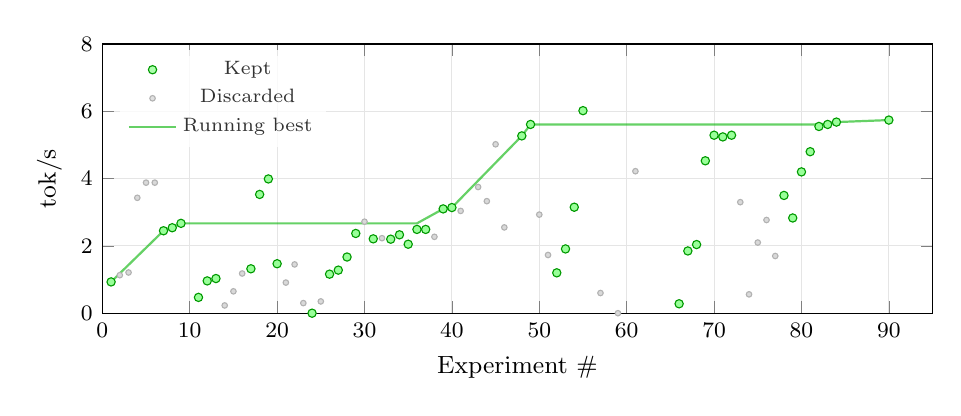
\begin{tikzpicture}
\begin{axis}[
    width=\columnwidth,
    height=5.0cm,
    xlabel={Experiment \#},
    ylabel={tok/s},
    xlabel style={font=\small},
    ylabel style={font=\small},
    tick label style={font=\footnotesize},
    xmin=0, xmax=95,
    ymin=0, ymax=8,
    grid=both,
    grid style={gray!20},
    legend style={font=\scriptsize, at={(0.02,0.98)}, anchor=north west, draw=none, fill=white, fill opacity=0.8},
]
% Kept experiments (green dots)
\addplot+[only marks, mark=*, mark size=1.5pt, green!60!black, mark options={fill=green!40}] coordinates {
    (1,0.93) (7,2.45) (8,2.54) (9,2.67) (10,36.95) (11,0.47) (12,0.96)
    (13,1.03) (17,1.32) (18,3.53) (19,3.99) (20,1.47)
    (24,0.00) (26,1.16) (27,1.28) (28,1.67) (29,2.37) (31,2.21) (33,2.20)
    (34,2.33) (35,2.05) (36,2.49) (37,2.49) (39,3.10) (40,3.14)
    (48,5.27) (49,5.61)
    (52,1.20) (53,1.91) (54,3.15) (55,6.02)
    (63,8.71) (64,13.90) (65,14.40) (66,0.28) (67,1.85) (68,2.04)
    (69,4.53) (70,5.29) (71,5.24) (72,5.29)
    (78,3.50) (79,2.83) (80,4.20) (81,4.80)
    (82,5.55) (83,5.61) (84,5.68) (90,5.74)
};
% Discarded experiments (gray dots)
\addplot+[only marks, mark=*, mark size=1pt, gray!60, mark options={fill=gray!30}] coordinates {
    (2,1.13) (3,1.21) (4,3.43) (5,3.88) (6,3.88)
    (14,0.23) (15,0.65) (16,1.18)
    (21,0.91) (22,1.45) (23,0.30)
    (25,0.35) (30,2.72) (32,2.23)
    (38,2.27) (41,3.04)
    (42,10.10) (43,3.75) (44,3.33) (45,5.02) (46,2.55) (47,10.10)
    (50,2.93) (51,1.73)
    (57,0.60) (59,0.00) (61,4.22)
    (73,3.30)
    (74,0.56) (75,2.10) (76,2.77) (77,1.70)
};
% Running best line for kept experiments
\addplot+[no marks, thick, green!70!black, opacity=0.6] coordinates {
    (1,0.93) (7,2.45) (8,2.54) (9,2.67) (36,2.67) (39,3.10) (40,3.14)
    (48,5.27) (49,5.61) (82,5.61) (84,5.68) (90,5.74)
};
\legend{Kept, Discarded, Running best}
\end{axis}
\end{tikzpicture}
\caption{Optimization trajectory across 90+ experiments. Green: kept (improved or informative). Gray: discarded (regressed or broken output). The spike at experiment 64 (13.9\,tok/s) was a GPU-only benchmark without attention---not representative of end-to-end performance. The running-best line shows genuine end-to-end progress from 0.93 to 5.74\,tok/s.}
\label{fig:journey}
\end{figure}

The trajectory reveals several phase transitions:
\begin{enumerate}[leftmargin=*,itemsep=2pt]
    \item \textbf{Experiments 1--20} (MLX era): Establishing baselines, fixing cache eviction races, building the profiling infrastructure. Best: 3.14\,tok/s with MLX.
    \item \textbf{Experiments 20--40} (Optimization plateau): Diminishing returns from MLX-level optimizations. Expert pruning ($K$=4) was the key unlock.
    \item \textbf{Experiments 40--55} (Two-pass experiments): Attempting to overlap routing and I/O across layers. Achieved 6\,tok/s but with degraded output quality.
    \item \textbf{Experiments 55--72} (Metal engine): Complete rewrite in Objective-C/Metal. Initial GPU-only benchmarks showed 14\,tok/s; end-to-end with correct attention reached 5.29\,tok/s.
    \item \textbf{Experiments 72--84} (2-bit + polish): Requantization, BLAS acceleration, fused pipelines. Reached 5.68\,tok/s.
    \item \textbf{Experiments 84+} (Trust the OS): Removed Metal LRU cache and F\_NOCACHE. C tokenizer, batch prefill, session caching. Final: 5.74\,tok/s.
\end{enumerate}

Notably, 42\% of experiments were discarded.
The most common failure mode was \emph{broken output}---optimizations that improved throughput but silently corrupted the computation (cache eviction races, routing-buffer mapping bugs, incorrect attention).
This underscores the importance of always verifying output quality, not just speed.

% ============================================================================
% 7. Discussion & Future Work
% ============================================================================
\section{Discussion and Future Work}

\paragraph{1-bit and ternary experts.}
Our 2-bit requantization reduced expert size by 44\%.
Ternary ($\{-1, 0, +1\}$) or binary quantization could push further, potentially halving I/O again.
The question is whether MoE expert weights tolerate this level of compression.
Recent work on BitNet suggests that models \emph{trained} at low precision perform well, but \emph{post-training} quantization below 2 bits typically requires mixed-precision approaches.

\paragraph{ANE co-processing.}
The Apple Neural Engine provides $\sim$16\,TFLOPS of FP16 compute on M3 Max, currently unused by our system.
Offloading attention operations to the ANE while the GPU handles expert MoE could improve parallelism.
The challenge is the ANE's restricted programming model: it requires CoreML or MIL-format models and does not support the dynamic control flow (top-$K$ routing, variable expert selection) that MoE inference demands.

\paragraph{Speculative decoding.}
Using Qwen3.5-35B-A3B (which fits in DRAM at 37\,tok/s) as a draft model for the 397B verifier is appealing but our initial experiment showed only 33\% acceptance rate at $K$=4 draft tokens, yielding a net 4.5$\times$ slowdown.
The draft model's routing decisions diverge significantly from the 397B model's, limiting acceptance.
A better approach might be self-speculative decoding using the 397B model with $K$=1 (very fast, very low quality) as the draft.

\paragraph{Multi-device inference.}
Two M3 Max laptops connected via Thunderbolt could each handle 30 layers, halving per-device I/O and potentially doubling throughput.
Apple's unified memory model extends across Thunderbolt-connected devices via the Apple Fabric bus, though latency and bandwidth characteristics of inter-device transfers remain to be characterized.

\paragraph{Applicability to other MoE models.}
Our approach generalizes to any MoE model where expert weights dominate total parameters.
DeepSeek-V3 (671B, 37B active) is an obvious candidate---at 2-bit expert quantization, the expert weights would be $\sim$200\,GB, within range of our streaming approach with modest SSD capacity requirements.

% ============================================================================
% 8. Conclusion
% ============================================================================
\section{Conclusion}

We have demonstrated that the Mixture-of-Experts architecture's fundamental sparsity enables running models vastly exceeding DRAM capacity on consumer hardware via NVMe SSD streaming.
Qwen3.5-397B-A17B---a model with 397 billion total parameters---runs at 5.74 tokens per second on a laptop with 48\,GB of RAM, using only 6.5\,GB of resident memory.

The key enabling insights are:
\begin{enumerate}[leftmargin=*,itemsep=2pt]
    \item MoE models need only 2--4\% of their expert weights per token, making SSD streaming viable.
    \item 2-bit requantization of already-quantized expert weights incurs negligible quality loss (RMSE $<$ 0.003) while reducing I/O by 44\%.
    \item A fused Metal GPU pipeline with deferred expert dispatch minimizes CPU--GPU synchronization overhead.
    \item \texttt{pread()} outperforms memory-mapped I/O by 5$\times$ for large, non-sequential expert reads.
    \item Expert pruning from $K$=10 to $K$=4 provides 2.6$\times$ speedup with no quality degradation, with a sharp quality cliff at $K$=3.
    \item Trusting the OS page cache---removing all application-level caching and I/O bypass flags---yields the best performance, because macOS's unified buffer cache is hardware-aware and avoids the memory compressor thrashing caused by GPU-visible Metal buffers.
\end{enumerate}

Our system's throughput is I/O-bound, suggesting that further gains require either faster storage or reduced I/O through better quantization.
With NVMe bandwidth improving $\sim$20\% annually, interactive inference of 400B+ parameter models on consumer laptops is rapidly becoming practical.

All code, weight preparation scripts, and the complete experiment log (90 experiments with git hashes) are available as supplementary material.

% ============================================================================
% Acknowledgments
% ============================================================================
\section*{Acknowledgments}
This work was conducted entirely on a personal MacBook Pro using the autoresearch methodology~\cite{karpathy2025autoresearch}.
We thank the MLX team at Apple for their framework and the mlx-community for pre-quantized model weights.
The maderix/ANE project provided valuable reference material on Apple Neural Engine internals.

% ============================================================================
% References
% ============================================================================
\bibliographystyle{plain}
\begin{thebibliography}{10}

\bibitem{alizadeh2023llm}
K.~Alizadeh, I.~Mirzadeh, D.~Belenko, K.~Khatamifard, M.~Cho, C.~C.~Del~Mundo, M.~Rastegari, and M.~Farajtabar.
\newblock {LLM in a Flash: Efficient Large Language Model Inference with Limited Memory}.
\newblock \emph{arXiv preprint arXiv:2312.11514}, 2023.

\bibitem{yang2025qwen3}
A.~Yang, B.~Yang, B.~Zhang, C.~Hui, et~al.
\newblock {Qwen3 Technical Report}.
\newblock Technical report, Alibaba Group, 2025.

\bibitem{jiang2024mixtral}
A.~Q.~Jiang, A.~Sablayrolles, A.~Roux, A.~Mensch, et~al.
\newblock {Mixtral of Experts}.
\newblock \emph{arXiv preprint arXiv:2401.04088}, 2024.

\bibitem{frantar2022gptq}
E.~Frantar, S.~Ashkboos, T.~Hoefler, and D.~Alistarh.
\newblock {GPTQ: Accurate Post-Training Quantization for Generative Pre-trained Transformers}.
\newblock \emph{arXiv preprint arXiv:2210.17323}, 2022.

\bibitem{dettmers2023case}
T.~Dettmers, R.~Svirschevski, V.~Egiazarian, D.~Kuznedelev, E.~Frantar, S.~Ashkboos, A.~Borzunov, T.~Hoefler, and D.~Alistarh.
\newblock {The case for 4-bit precision: k-bit Inference Scaling Laws}.
\newblock In \emph{Advances in Neural Information Processing Systems (NeurIPS)}, 2023.

\bibitem{kwon2023efficient}
W.~Kwon, Z.~Li, S.~Zhuang, Y.~Sheng, L.~Zheng, C.~H.~Yu, J.~E.~Gonzalez, H.~Zhang, and I.~Stoica.
\newblock {Efficient Memory Management for Large Language Model Serving with PagedAttention}.
\newblock In \emph{Proceedings of the 29th Symposium on Operating Systems Principles (SOSP)}, 2023.

\bibitem{sheng2023flexgen}
Y.~Sheng, L.~Zheng, B.~Yuan, Z.~Li, M.~Ryabinin, D.~Y.~Fu, Z.~Xie, B.~Chen, C.~Barrett, J.~E.~Gonzalez, P.~Liang, C.~R\'{e}, I.~Stoica, and C.~Zhang.
\newblock {FlexGen: High-Throughput Generative Inference of Large Language Models with a Single GPU}.
\newblock In \emph{Proceedings of the 40th International Conference on Machine Learning (ICML)}, 2023.

\bibitem{mlx2023}
A.~Hannun, J.~Kastner, A.~Arfeen, R.~Yang, et~al.
\newblock {MLX: Efficient and Flexible Machine Learning on Apple Silicon}.
\newblock Technical report, Apple, 2023.

\bibitem{llamacpp}
G.~Gerganov et~al.
\newblock {llama.cpp: Port of Facebook's LLaMA model in C/C++}.
\newblock \url{https://github.com/ggerganov/llama.cpp}, 2023.

\bibitem{rajbhandari2021zero}
S.~Rajbhandari, O.~Ruwase, J.~Rasley, S.~Smith, and Y.~He.
\newblock {ZeRO-Infinity: Breaking the GPU Memory Wall for Extreme Scale Deep Learning}.
\newblock In \emph{Proceedings of the International Conference for High Performance Computing, Networking, Storage and Analysis (SC)}, 2021.

\bibitem{karpathy2025autoresearch}
A.~Karpathy.
\newblock {The Unreasonable Effectiveness of Autoresearch}.
\newblock Blog post, 2025.

\end{thebibliography}

% ============================================================================
% Appendix
% ============================================================================
\appendix

\section{Model Architecture Details}

\begin{table}[h]
\centering
\small
\caption{Qwen3.5-397B-A17B architecture constants.}
\begin{tabular}{@{}lr@{}}
\toprule
\textbf{Parameter} & \textbf{Value} \\
\midrule
Total parameters & 397B \\
Active parameters per token & 17B (default $K$=10) \\
Hidden dimension & 4096 \\
Number of layers & 60 \\
\quad Linear attention (GatedDeltaNet) & 45 \\
\quad Full attention (RoPE) & 15 \\
Full attention interval & Every 4th layer \\
Attention heads & 32 \\
KV heads (GQA) & 2 \\
Head dimension & 256 \\
Experts per layer & 512 \\
Default active experts ($K$) & 10 \\
Expert intermediate dim & 1024 \\
Shared expert intermediate dim & 1024 \\
Vocabulary size & 248{,}320 \\
Expert activation & SwiGLU \\
RoPE $\theta$ & $10^7$ \\
Partial rotary fraction & 0.25 \\
Conv kernel (linear attn) & 4 \\
\bottomrule
\end{tabular}
\end{table}

\section{2-Bit Expert Binary Layout}

Each expert at 2-bit precision occupies exactly 3{,}932{,}160 bytes with the following contiguous layout:

\begin{table}[h]
\centering
\small
\caption{2-bit expert binary layout. Offsets in bytes from expert start.}
\begin{tabular}{@{}lrrr@{}}
\toprule
\textbf{Component} & \textbf{Offset} & \textbf{Size} & \textbf{Shape} \\
\midrule
gate weights (uint32) & 0 & 1{,}048{,}576 & [1024, 256] \\
gate scales (bf16) & 1{,}048{,}576 & 131{,}072 & [1024, 64] \\
gate biases (bf16) & 1{,}179{,}648 & 131{,}072 & [1024, 64] \\
up weights (uint32) & 1{,}310{,}720 & 1{,}048{,}576 & [1024, 256] \\
up scales (bf16) & 2{,}359{,}296 & 131{,}072 & [1024, 64] \\
up biases (bf16) & 2{,}490{,}368 & 131{,}072 & [1024, 64] \\
down weights (uint32) & 2{,}621{,}440 & 1{,}048{,}576 & [4096, 64] \\
down scales (bf16) & 3{,}670{,}016 & 131{,}072 & [4096, 16] \\
down biases (bf16) & 3{,}801{,}088 & 131{,}072 & [4096, 16] \\
\midrule
\textbf{Total} & & \textbf{3{,}932{,}160} & \\
\bottomrule
\end{tabular}
\end{table}

\section{Complete Experiment Log}

A selection of key experiments from our 90-experiment trajectory:

\begin{table*}[h]
\centering
\footnotesize
\caption{Selected experiments from the optimization trajectory. Full log (90 entries with git hashes) available in supplementary material.}
\begin{tabular}{@{}rlrrrl@{}}
\toprule
\textbf{\#} & \textbf{Status} & \textbf{tok/s} & \textbf{Mem (GB)} & \textbf{Description} \\
\midrule
1 & keep & 0.93 & 3.7 & First working 122B inference (selective expert I/O) \\
7 & keep & 2.45 & 10.5 & First correct output (LRU eviction race fix) \\
11 & keep & 0.47 & 20.6 & 397B MOONSHOT---first 397B inference ever on this hardware \\
13 & keep & 1.03 & 21.4 & 397B 50-token steady state (1.03 tok/s plateau) \\
28 & keep & 1.67 & 28.1 & $K$=6 expert pruning (40\% less I/O) \\
29 & keep & 2.37 & 28.2 & $K$=4 expert pruning (best cached config) \\
36 & keep & 2.49 & 5.5 & All 60 layers packed + no-cache + $K$=4 \\
40 & keep & 3.14 & 5.4 & Full stack MLX: packed + batch + lazy-eval + pipeline \\
42 & discard & 10.10 & 5.8 & Variable $K$=0: 10 tok/s but blank output \\
66 & keep & 0.28 & 5.5 & C/Metal engine: first coherent output \\
70 & keep & 5.29 & 5.5 & C/Metal: GPU norm + residual shaders, peak 5.29 \\
82 & keep & 5.55 & 5.5 & 2-bit experts: 5.55 sustained, quality verified \\
84 & keep & 5.68 & 5.5 & F\_NOCACHE + 2-bit: 5.68 avg, 5.91 peak \\
90 & keep & 5.74 & 5.5 & Trust OS: removed Metal LRU cache + F\_NOCACHE. New best. \\
\bottomrule
\end{tabular}
\end{table*}

\end{document}
